\documentclass{article}
\usepackage[T1]{fontenc}
\usepackage{lmodern}
\usepackage[polish]{babel}
\usepackage{graphicx}
\usepackage{float}
\usepackage{hyperref}

\usepackage[a4paper, margin=2.54cm]{geometry}

\title{Praca domowa 8\\Drzewa decyzyjne}
\author{Damian Jankowski s188597}

\begin{document}

\maketitle

\section{Wstęp}

Celem pracy domowej było zbudowanie drzewa decyzyjnego
odpowiadającego na pytanie, czy panują odpowiednie
warunki atmosferyczne do rozegrania meczu golfa.

Dane wejściowe to tabela zawierająca informacje o
pogodzie przez 14 dni oraz informacja, czy w danym
dniu powinno się grać. Prezentuje się ona następująco:

\begin{table}[H]
    \centering
    \begin{tabular}{|c|c|c|c|}
    \hline
    \textbf{Outlook} & \textbf{Humidity} & \textbf{Windy} & \textbf{Play golf} \\
    \hline
    \hline
    Rainy & High & False & No \\
    \hline
    Rainy & High & True & No \\
    \hline
    Overcast & High & False & Yes \\
    \hline
    Sunny & High & False & Yes \\
    \hline
    Sunny & Normal & False & Yes \\
    \hline
    Sunny & Normal & True & No \\
    \hline
    Overcast & Normal & True & Yes \\
    \hline
    Rainy & High & False & No \\
    \hline
    Rainy & Normal & False & Yes \\
    \hline
    Sunny & Normal & False & Yes \\
    \hline
    Rainy & Normal & True & Yes \\
    \hline
    Overcast & High & True & Yes \\
    \hline
    Overcast & Normal & False & Yes \\
    \hline
    Sunny & High & True & No \\
    \hline
    \end{tabular}
\end{table}

\section{Opis algorytmu}

Algorytm budowania drzewa decyzyjnego polega na
znalezieniu atrybutu, który najlepiej rozdziela
zbiór danych. Następnie dla każdej wartości
tego atrybutu tworzone są poddrzewa, które
zawierają tylko te dane, dla których wartość
tego atrybutu jest równa wartości węzła.

By znaleźć najlepszy atrybut, należy obliczyć
entropię dla każdego z nich. Entropia jest
miarą nieporządku w zbiorze danych. Im większa
wartość entropii, tym większy nieporządek.

Entropia obliczana jest ze wzoru:

\begin{equation}
    E = -\sum_{i=1}^{n} p_i \log_2 p_i
\end{equation}

W przypadku drzewa decyzyjnego, prawdobodobieństwo
$p_i$ jest równe liczbie wystąpień danej wartości
atrybutu w zbiorze danych podzielonej przez
liczbę wszystkich danych z tym atrybutem.

Następnie wyznacza się tzw. zysk,
który jest różnicą entropii atrybutu $S$
oraz ważonej wartości entropii dla kolejnych wartości
atrybutów. Atrybut, dla którego
zysk jest największy, jest najlepszym
kandydatem na atrybut korzenia drzewa.

\begin{equation}
    Gain(S, A) = Entropy(S) - \sum_{v \in Values(A)} \frac{|S_v|}{|S|} Entropy(S_v)
\end{equation}

\section{Obliczenia}

\begin{figure}[H]
    \centering
    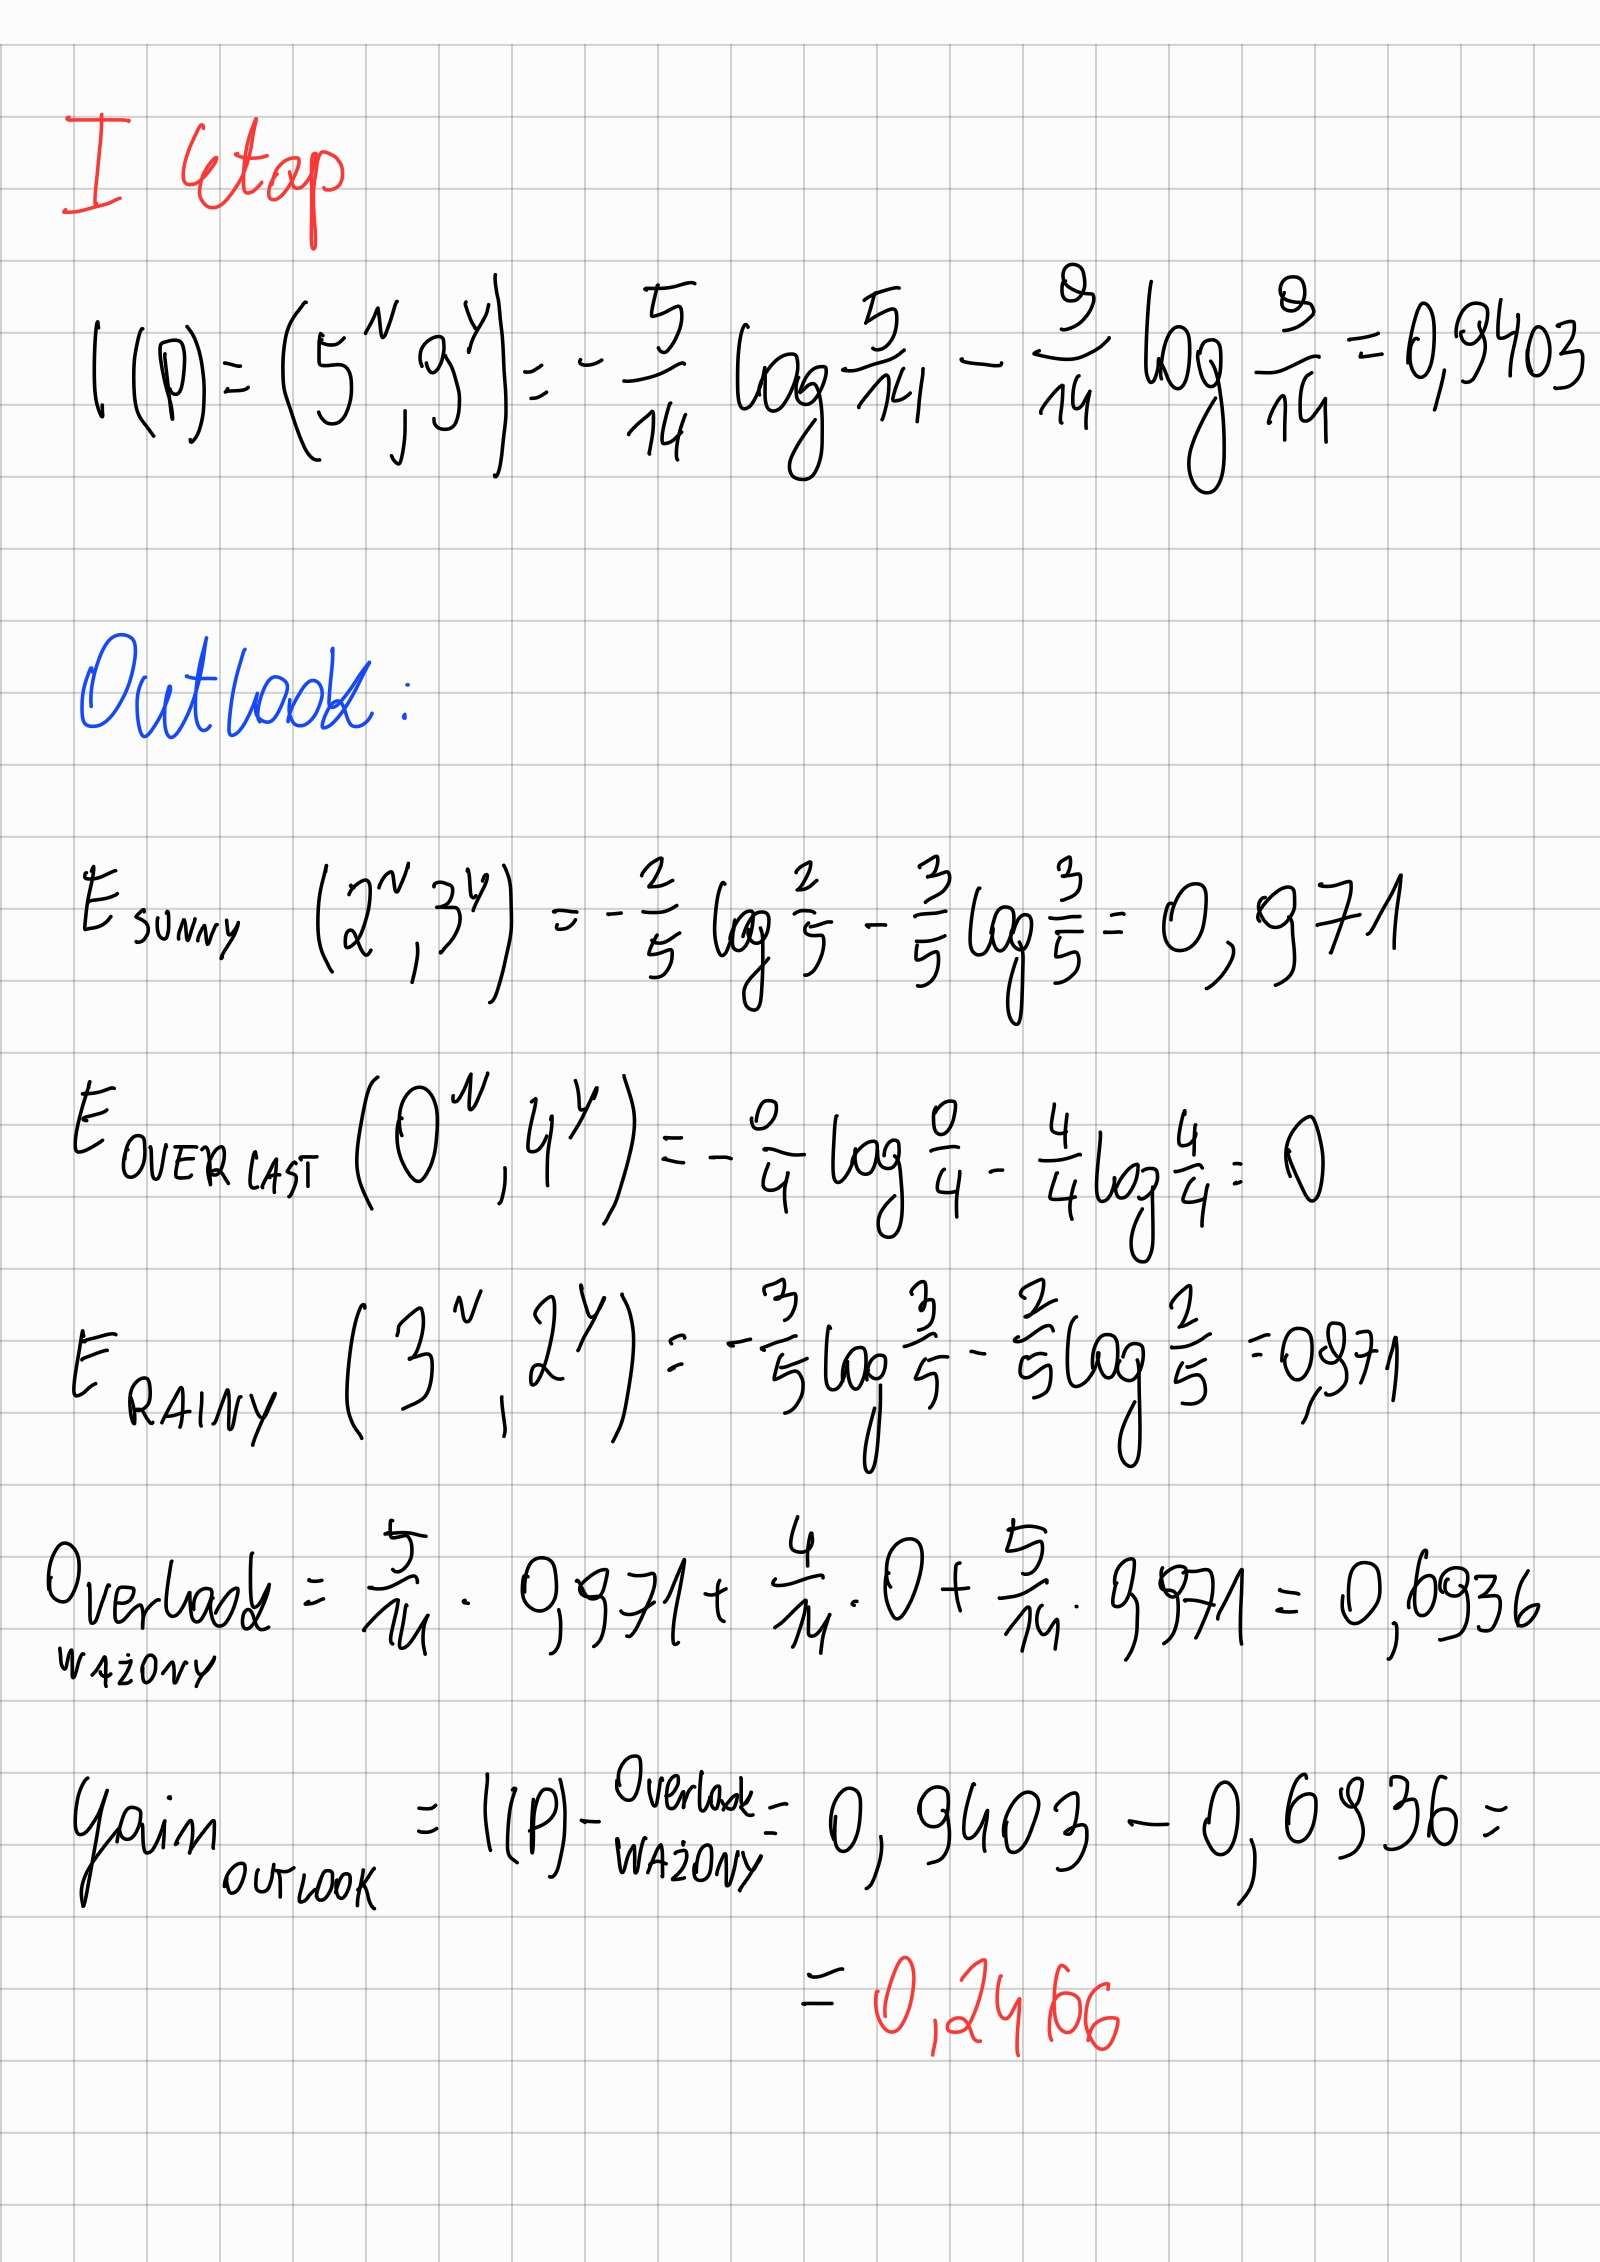
\includegraphics[width=\textwidth]{tree1.jpg}
\end{figure}

\begin{figure}[H]
    \centering
    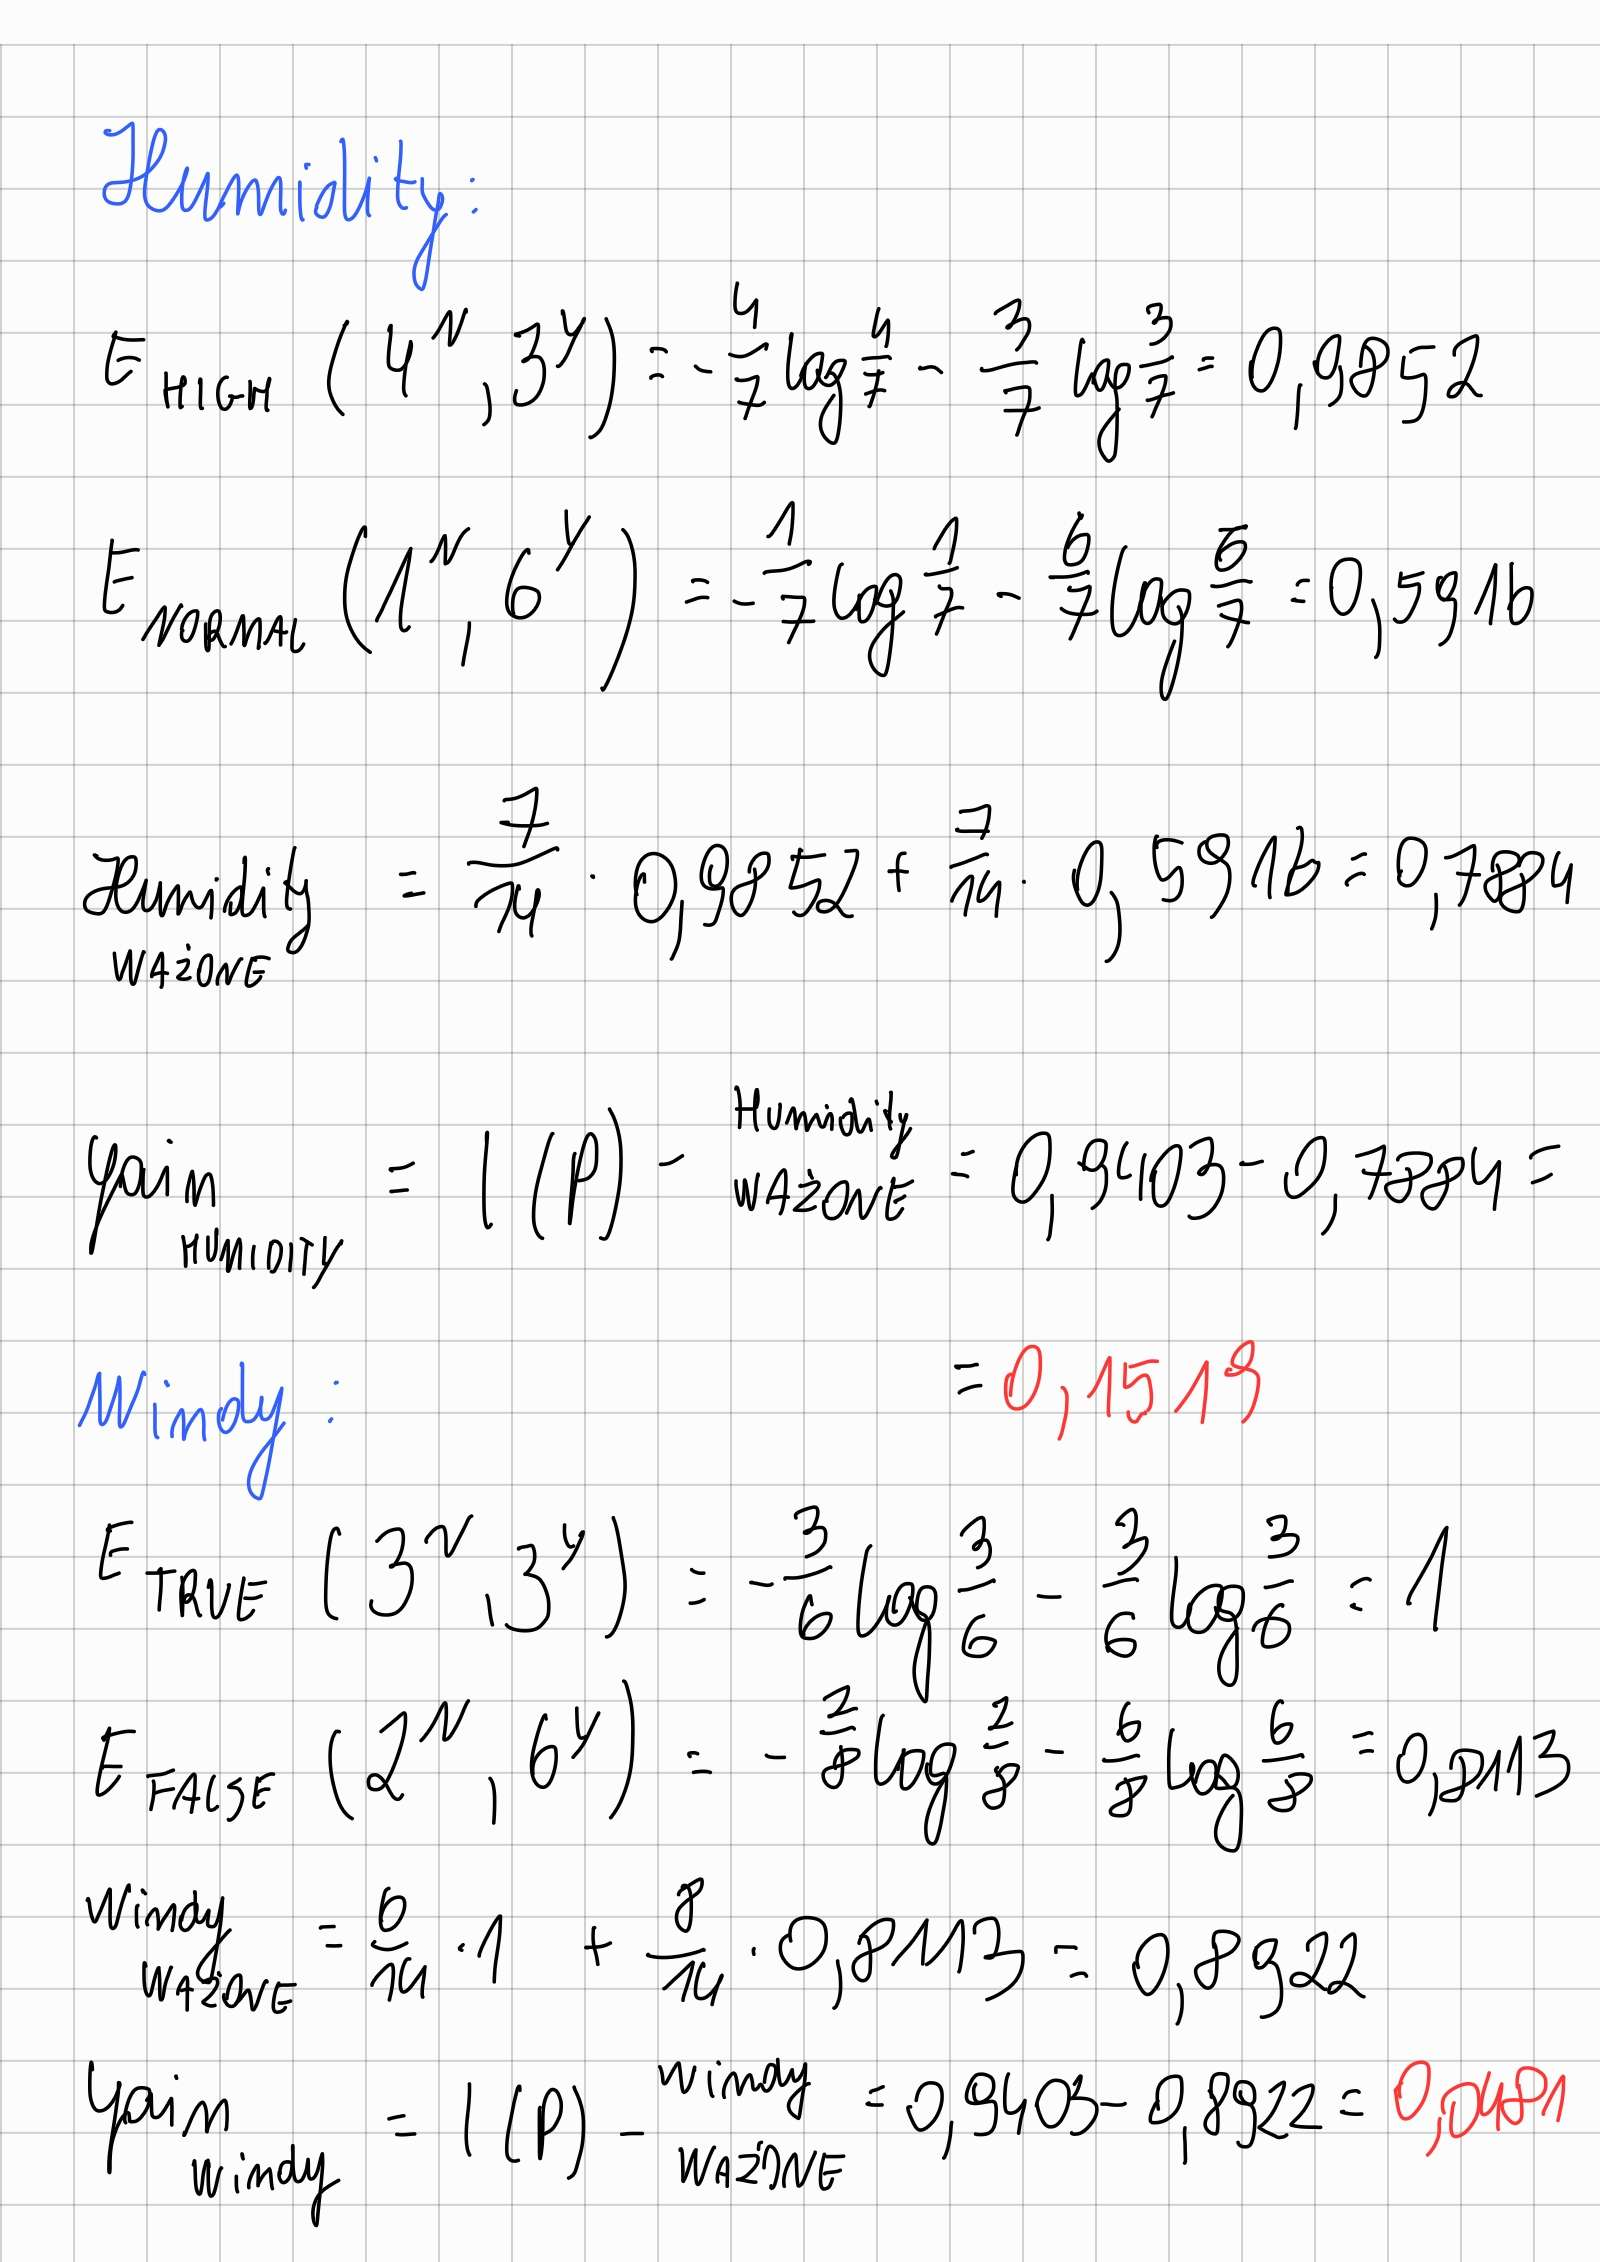
\includegraphics[width=\textwidth]{tree2.jpg}
\end{figure}

\begin{figure}[H]
    \centering
    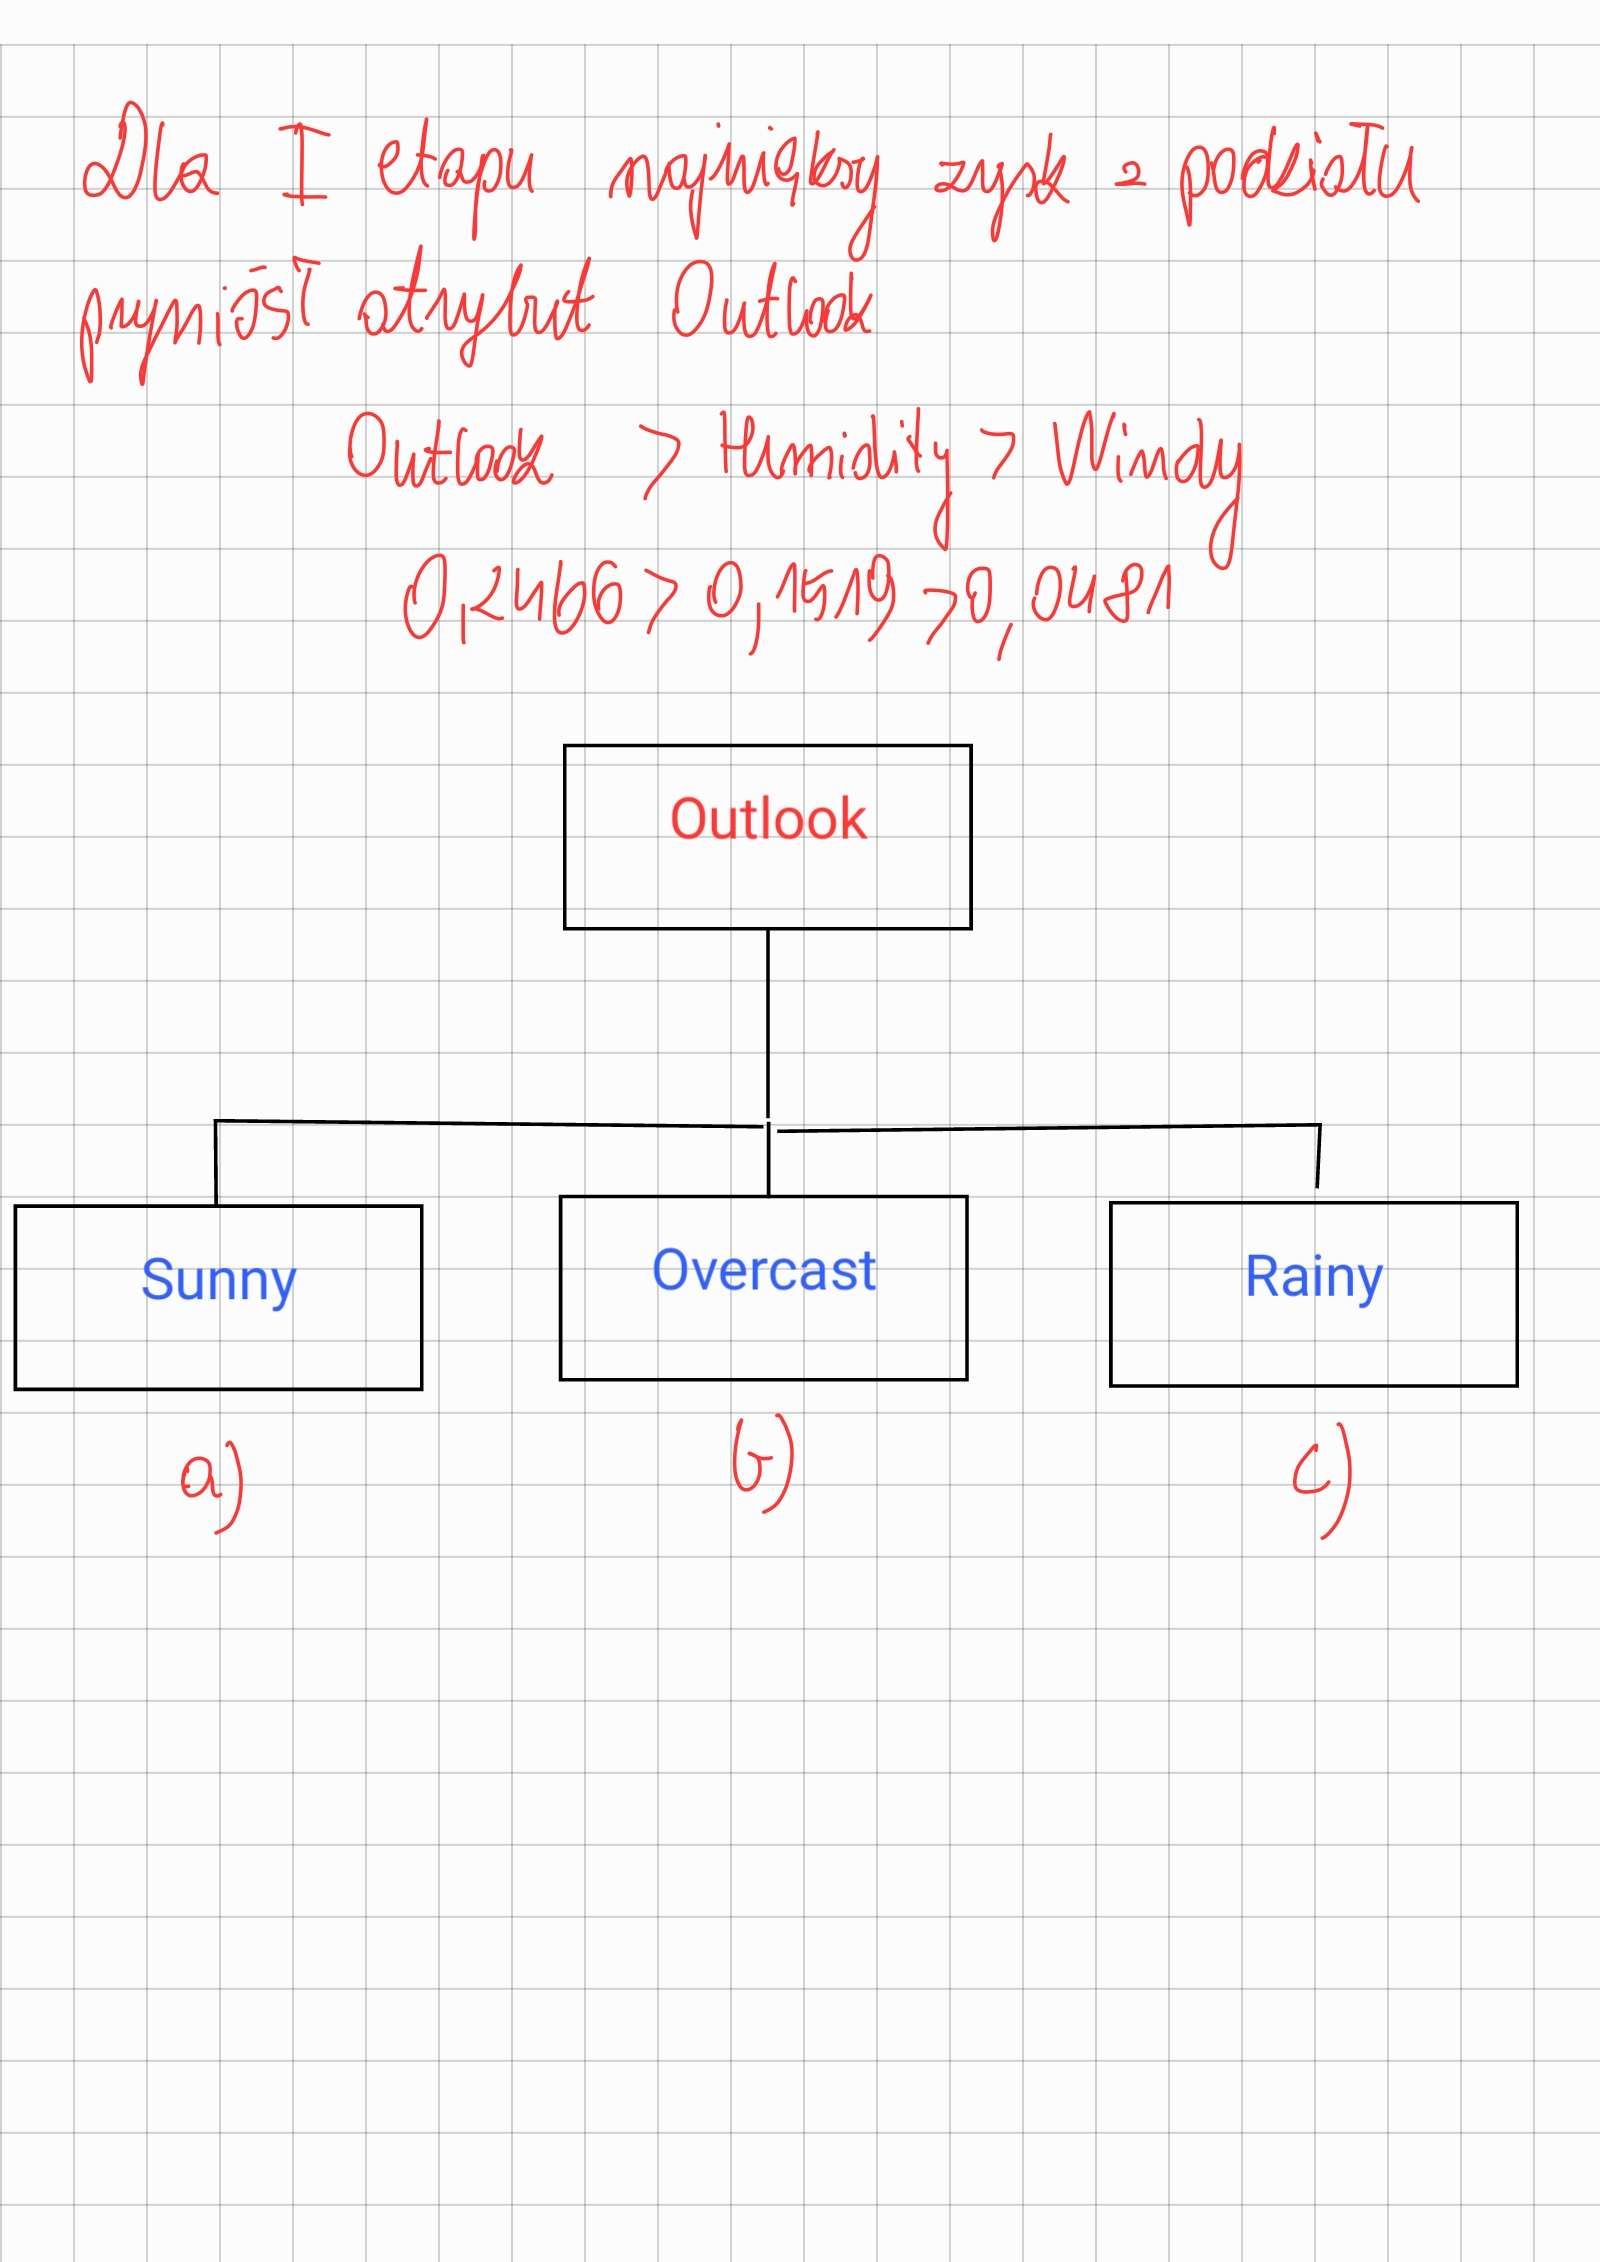
\includegraphics[width=\textwidth]{tree3.jpg}
\end{figure}

\begin{figure}[H]
    \centering
    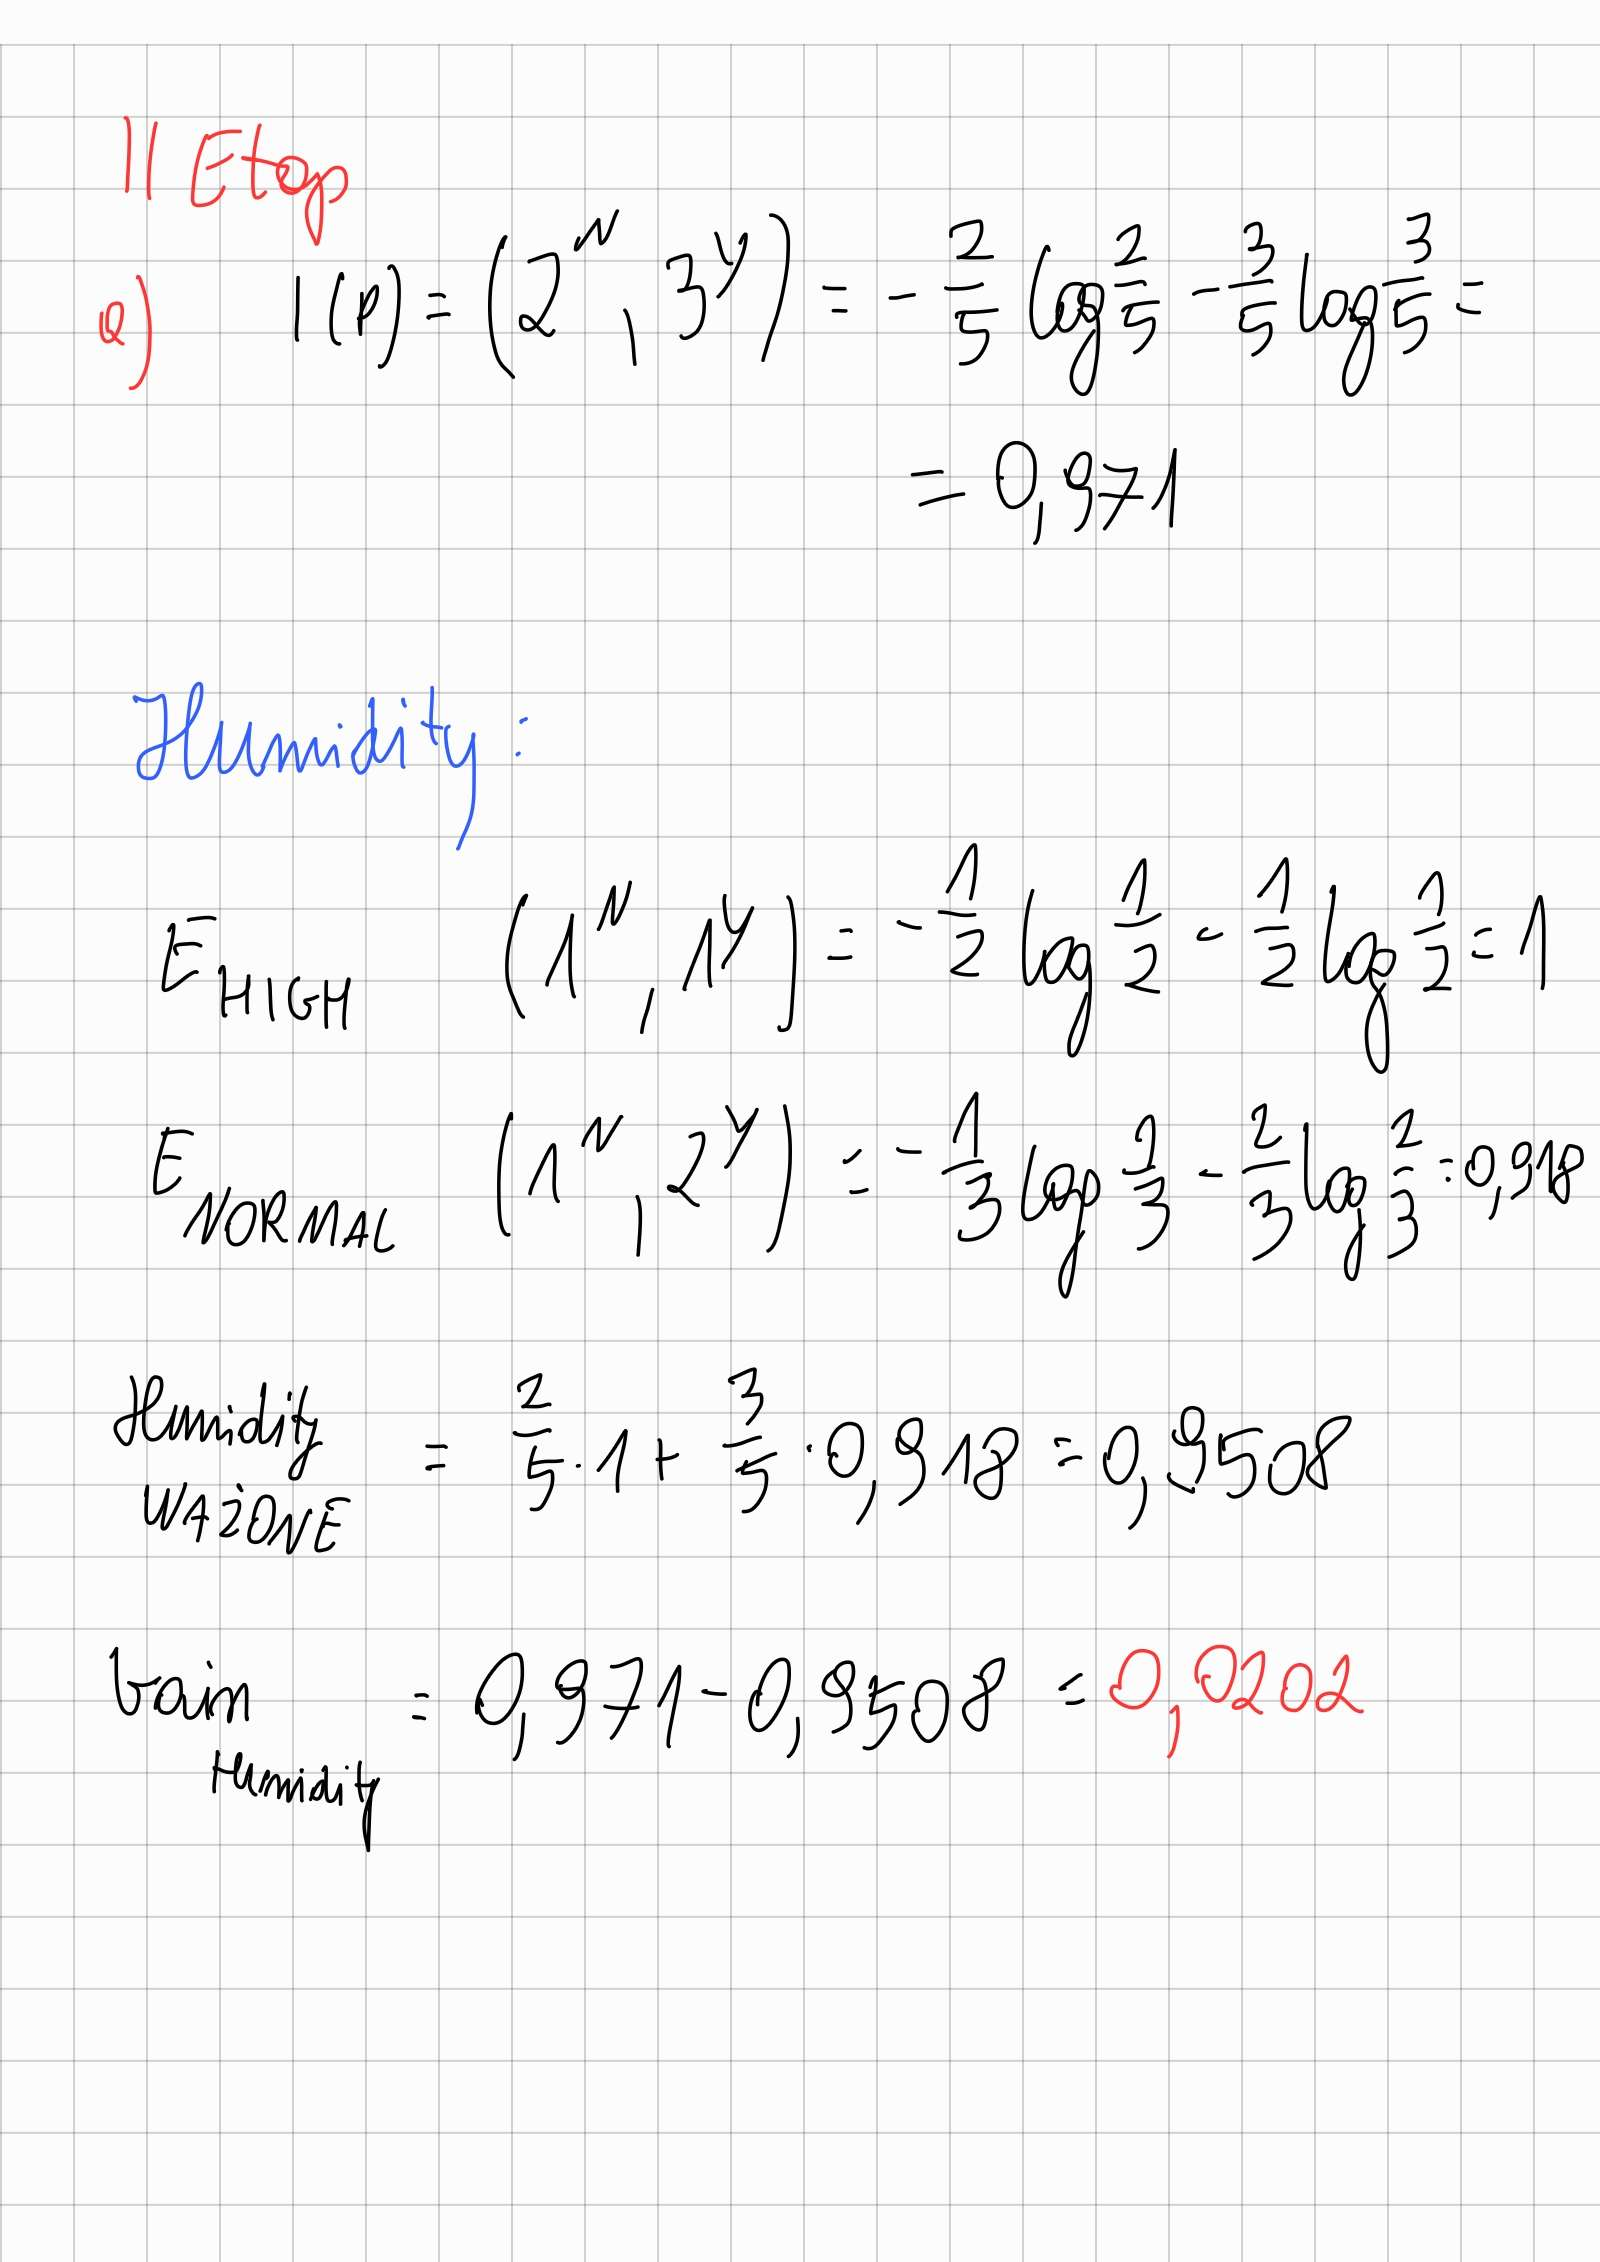
\includegraphics[width=\textwidth]{tree4.jpg}
\end{figure}

\begin{figure}[H]
    \centering
    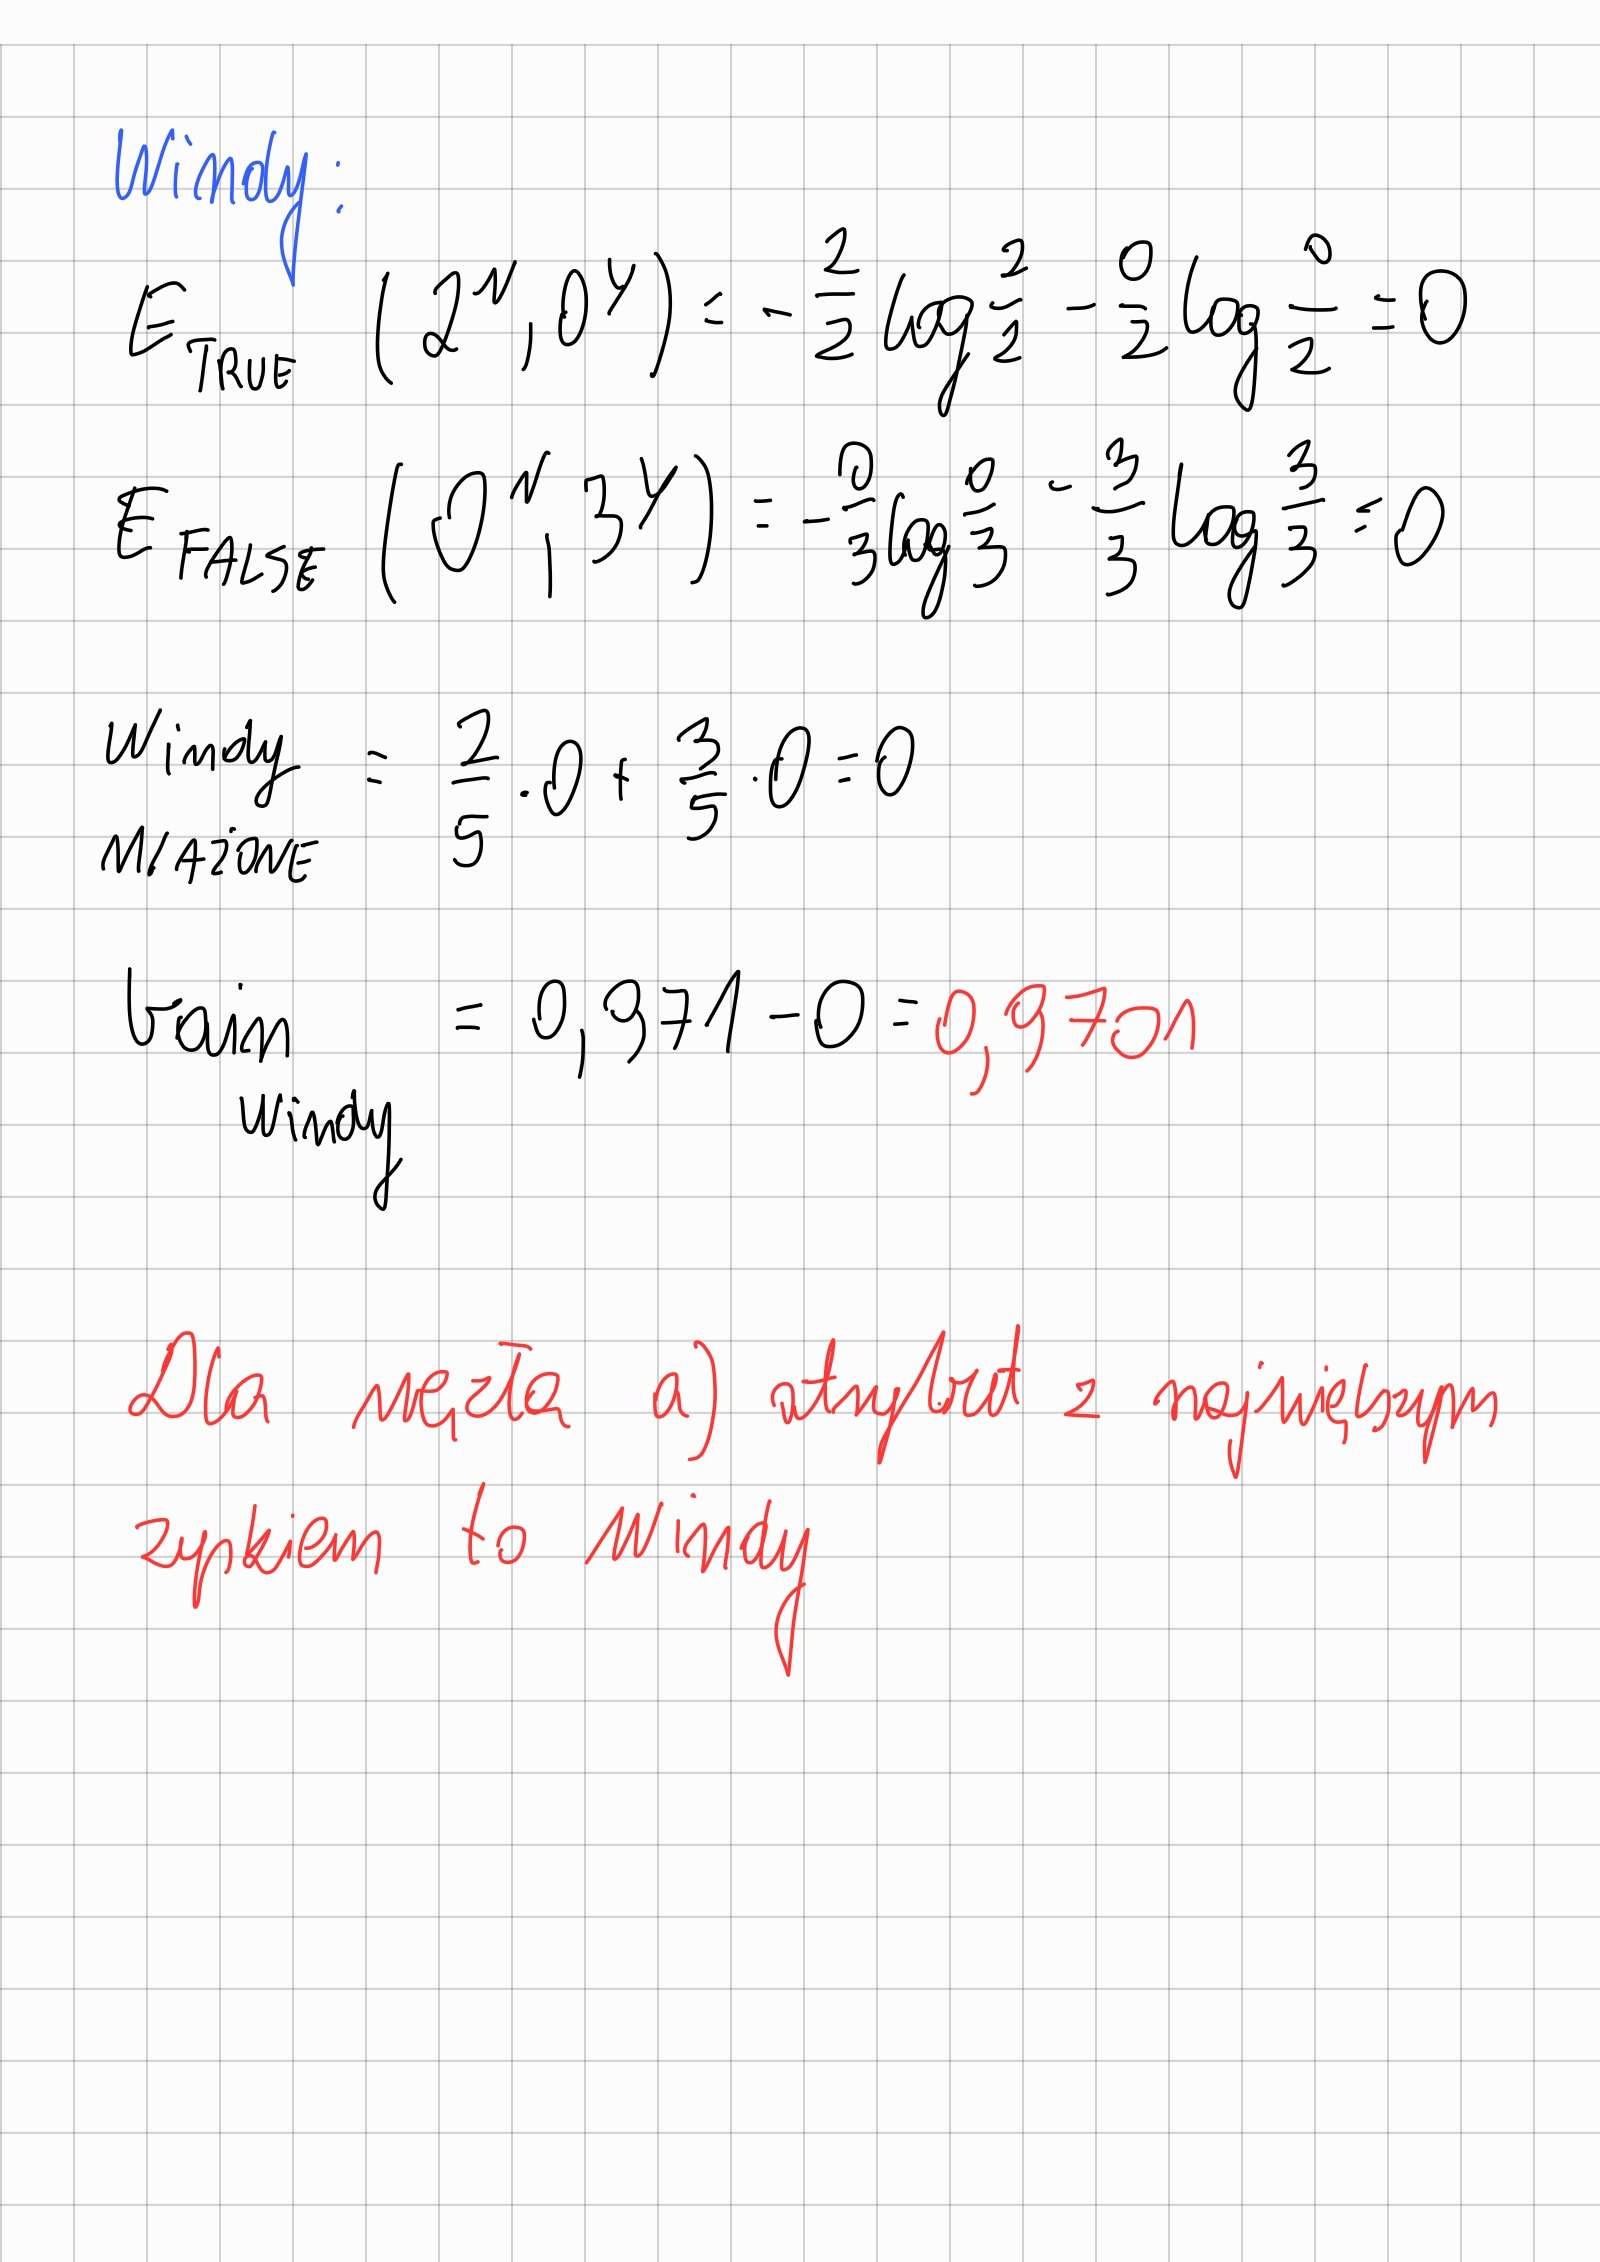
\includegraphics[width=\textwidth]{tree5.jpg}
\end{figure}

\begin{figure}[H]
    \centering
    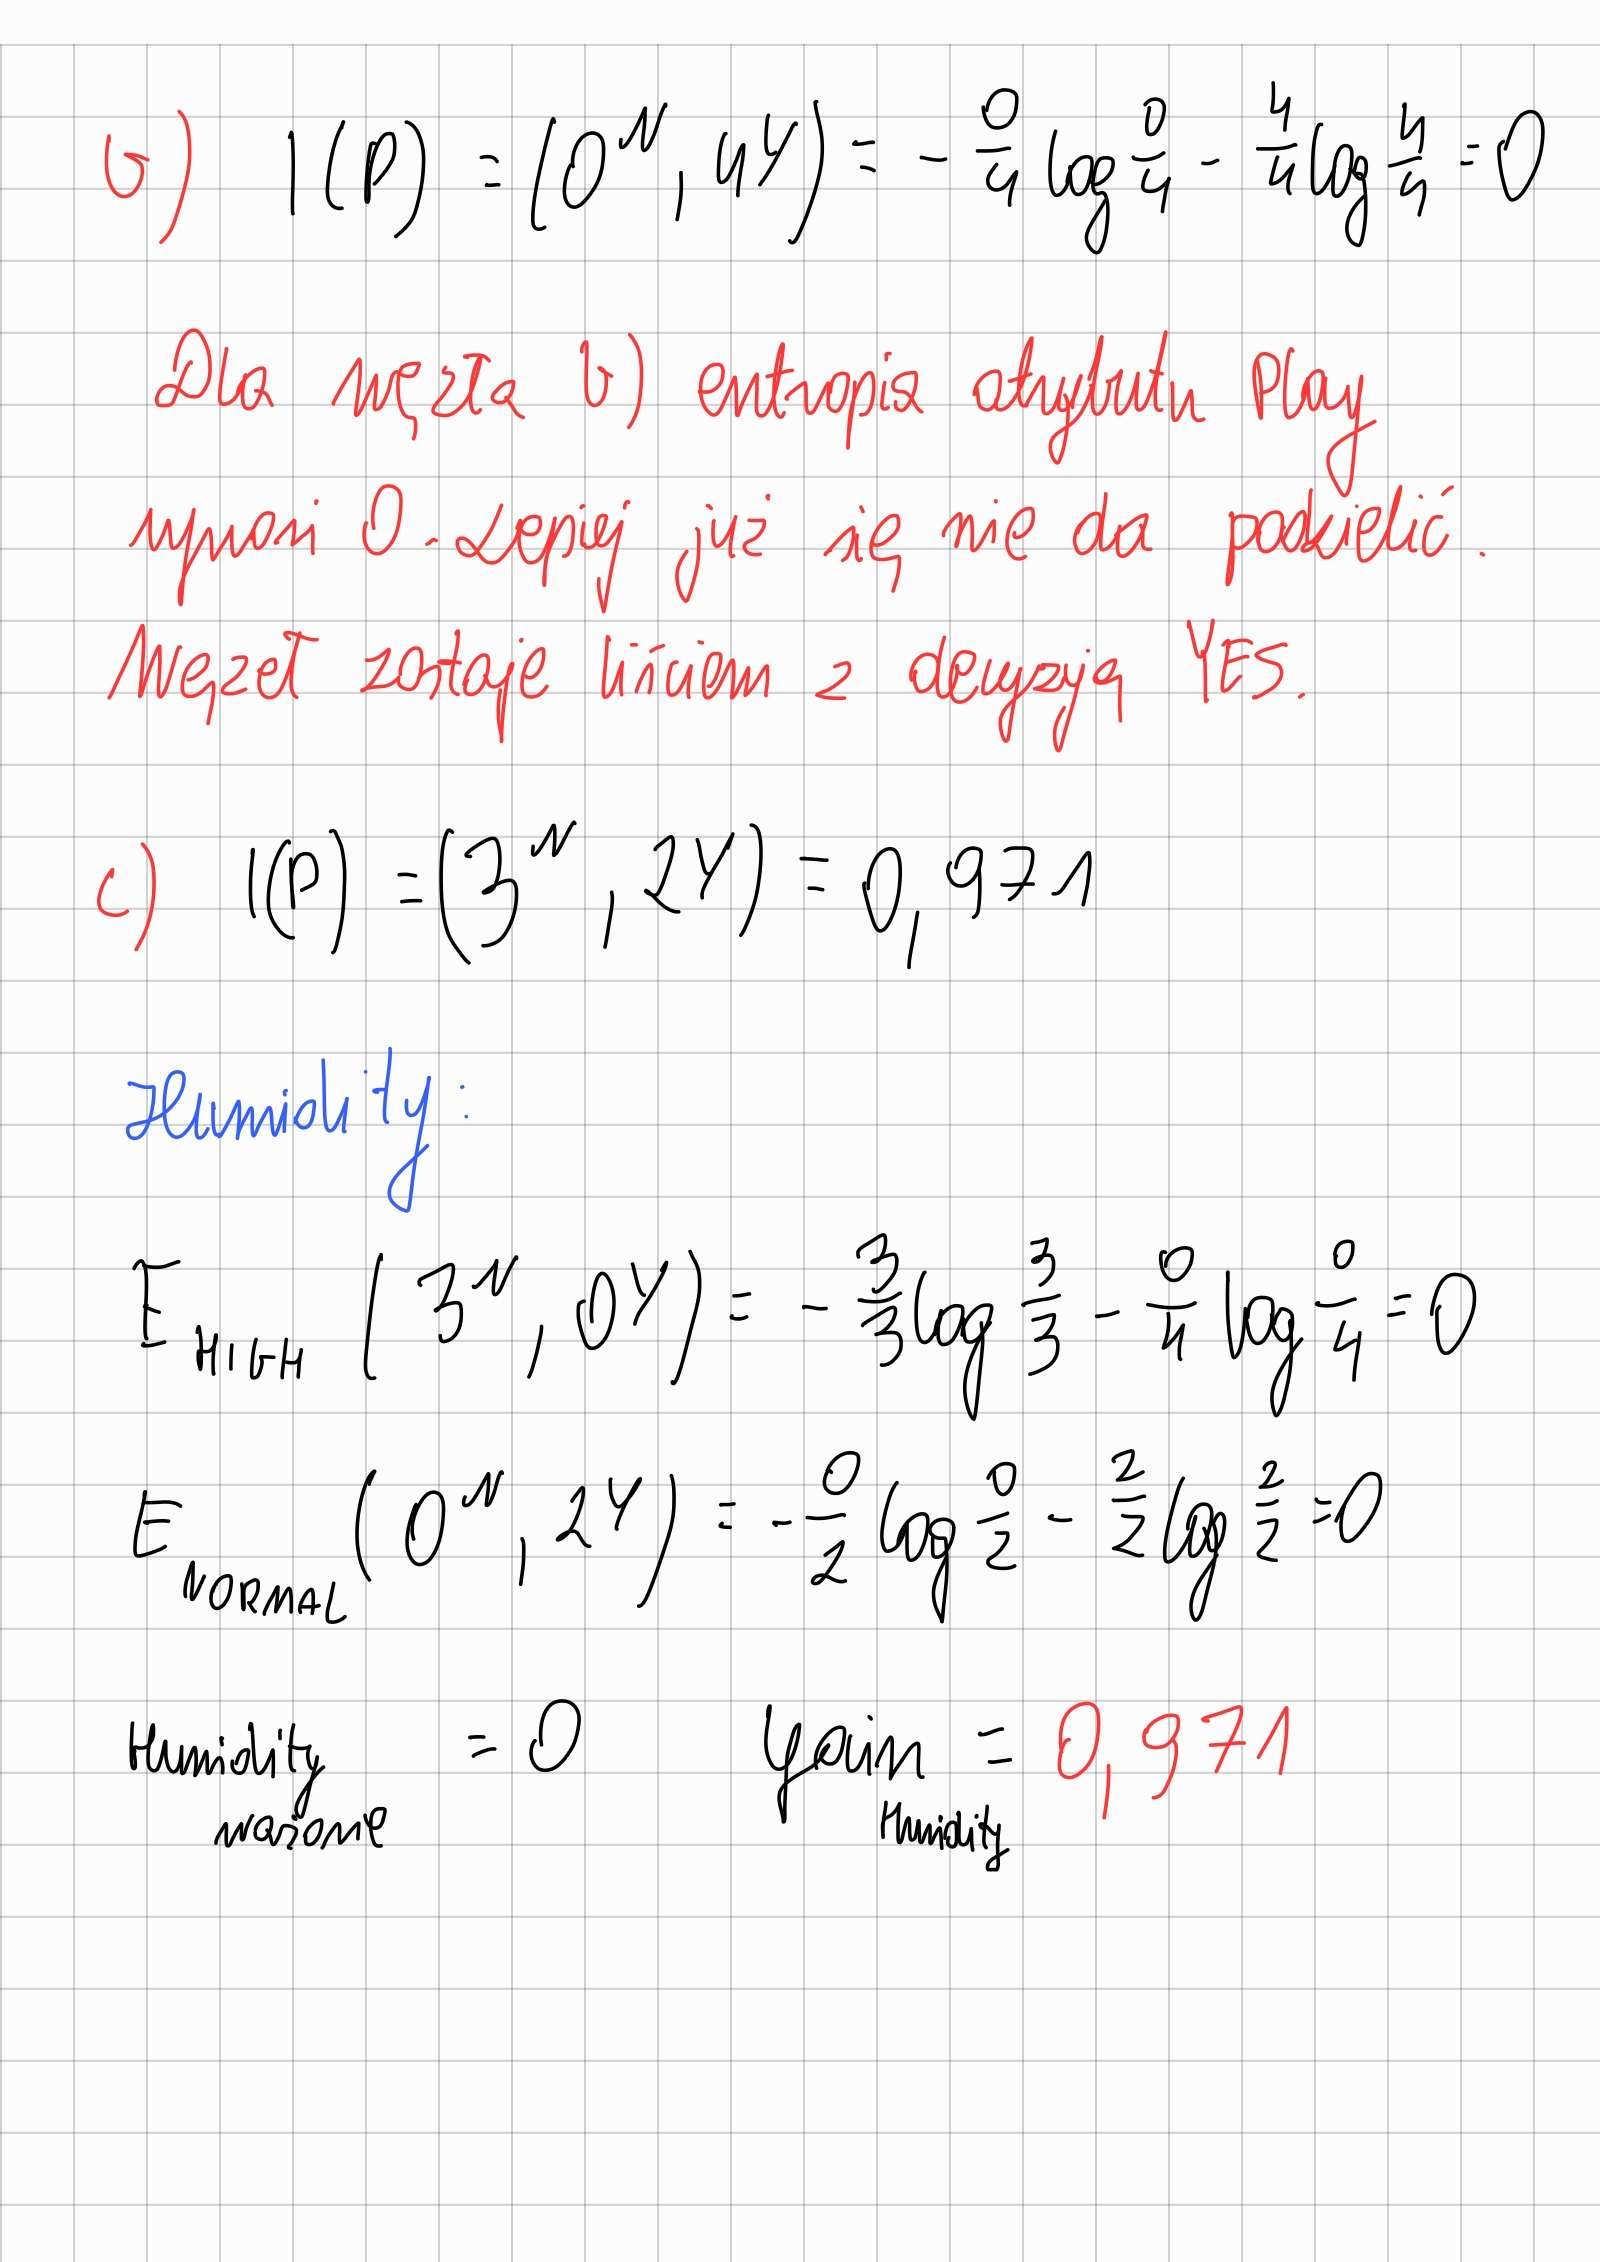
\includegraphics[width=\textwidth]{tree6.jpg}
\end{figure}

\begin{figure}[H]
    \centering
    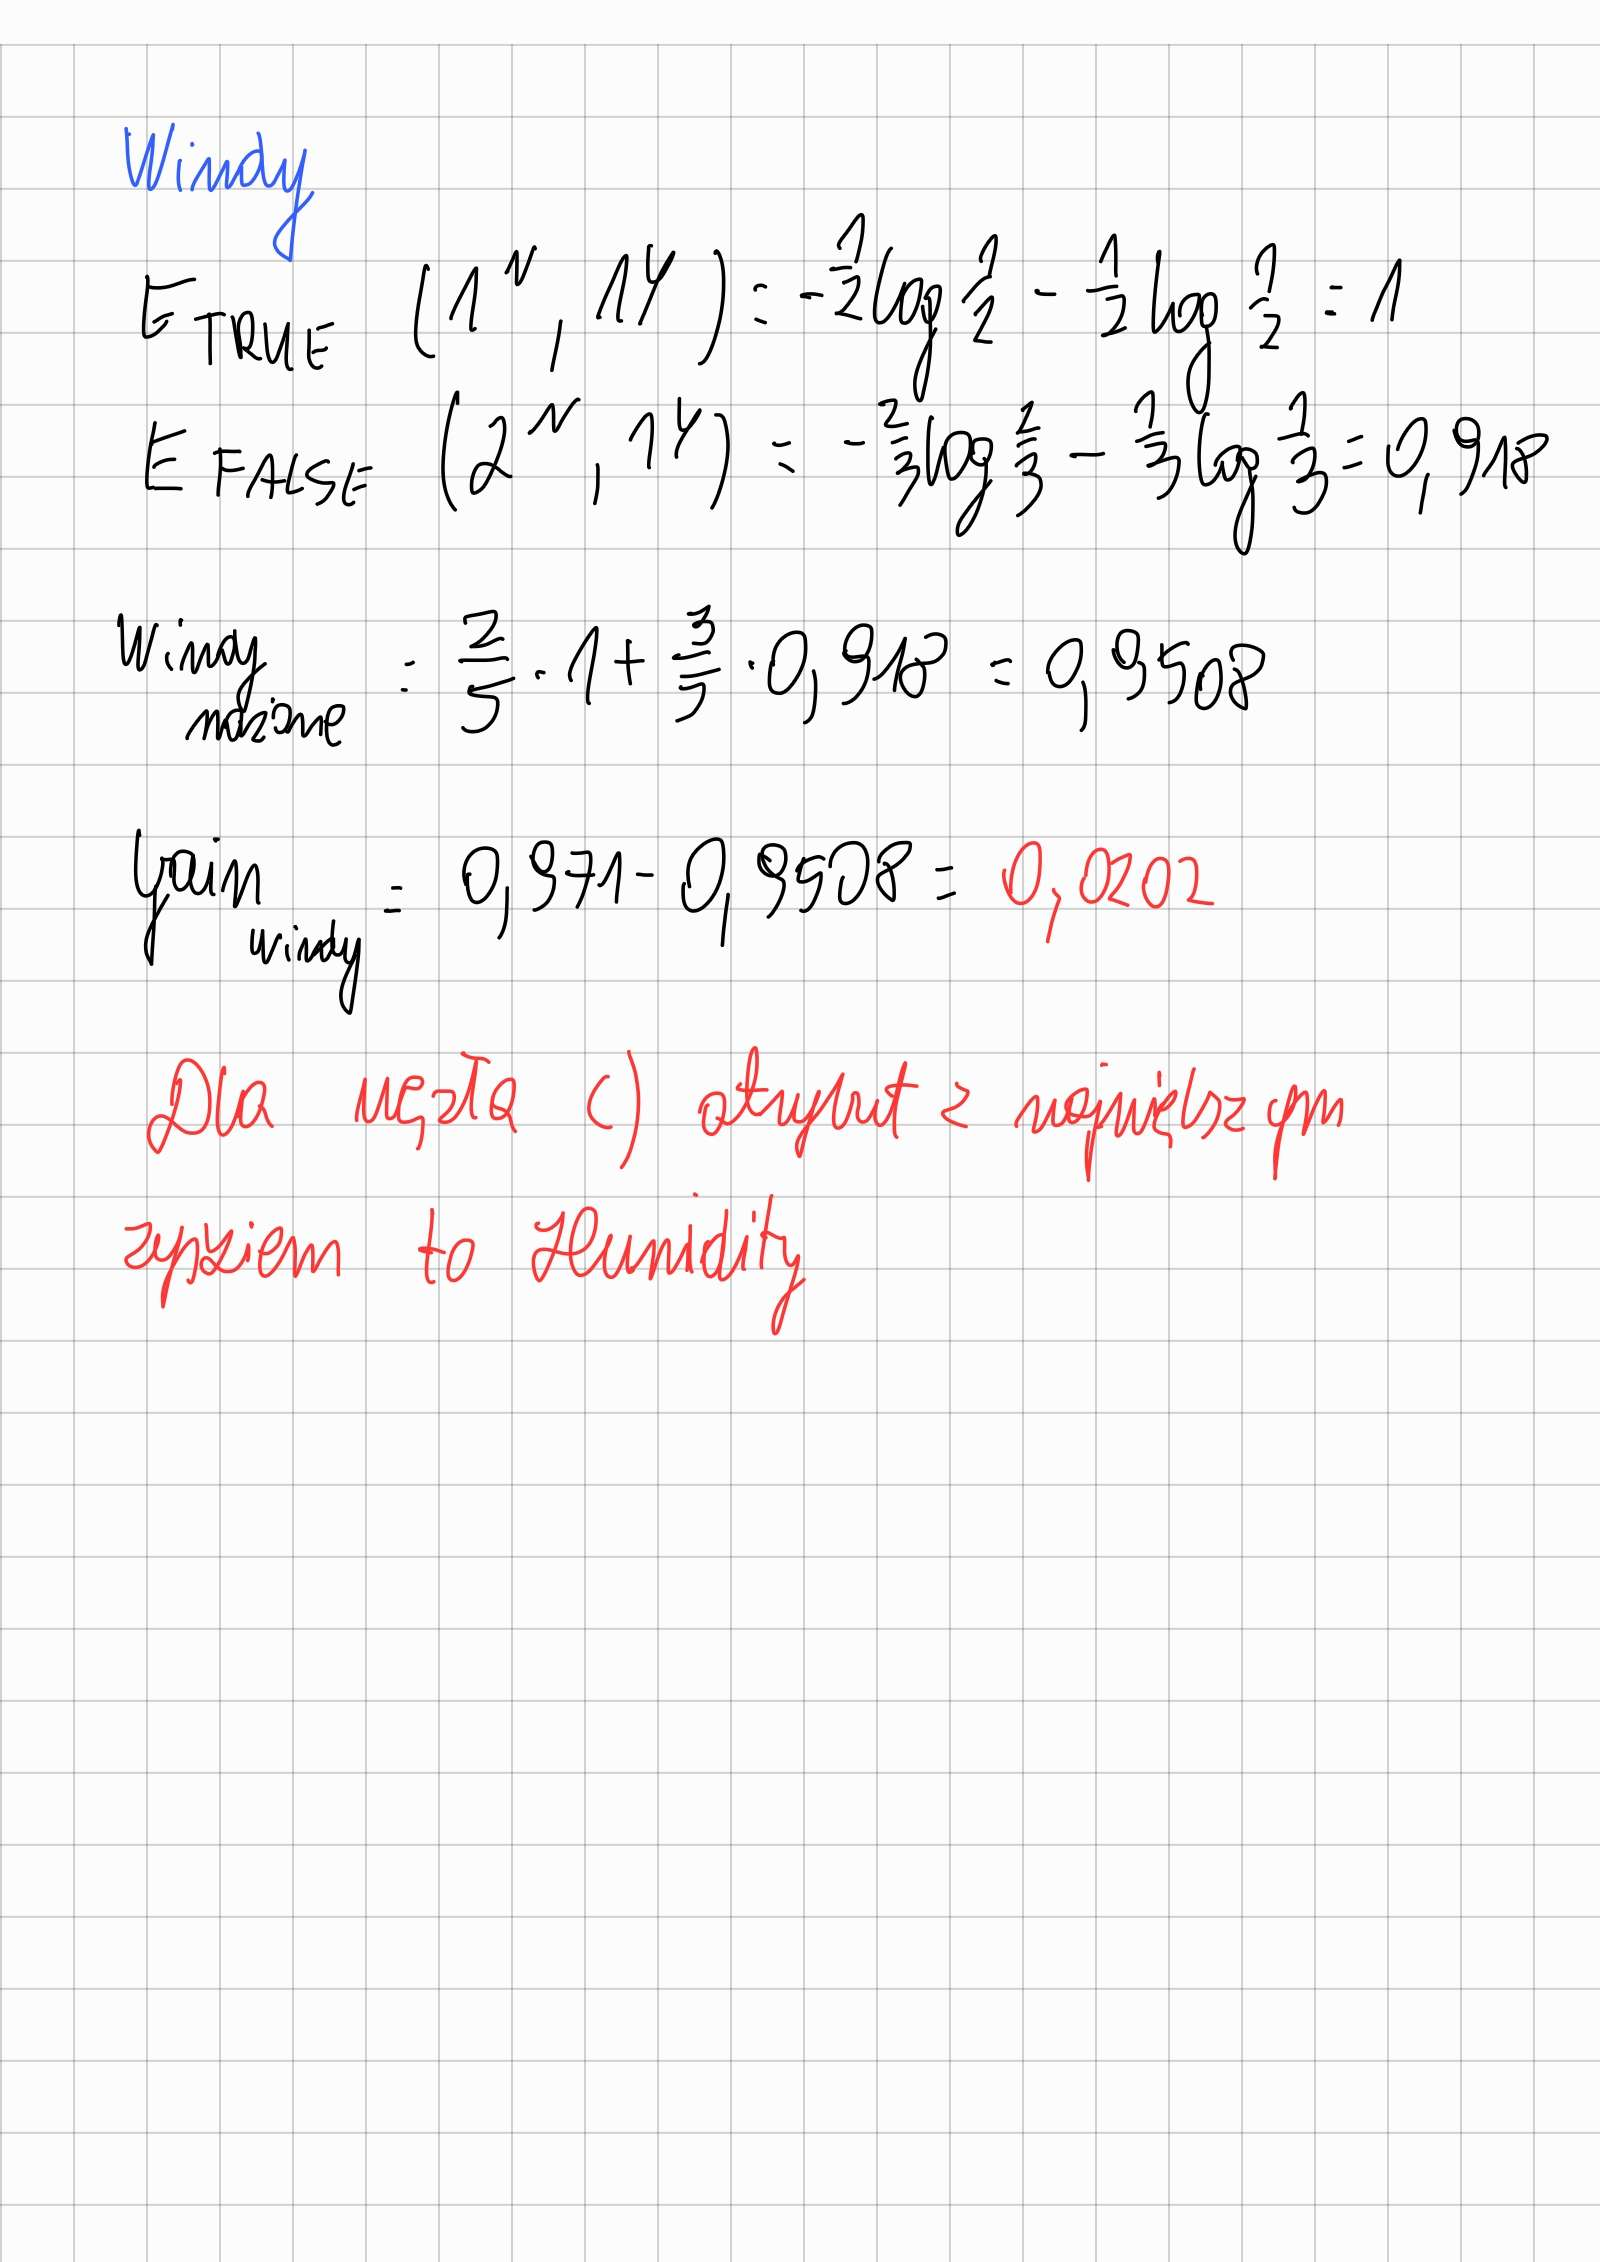
\includegraphics[width=\textwidth]{tree7.jpg}
\end{figure}

\begin{figure}[H]
    \centering
    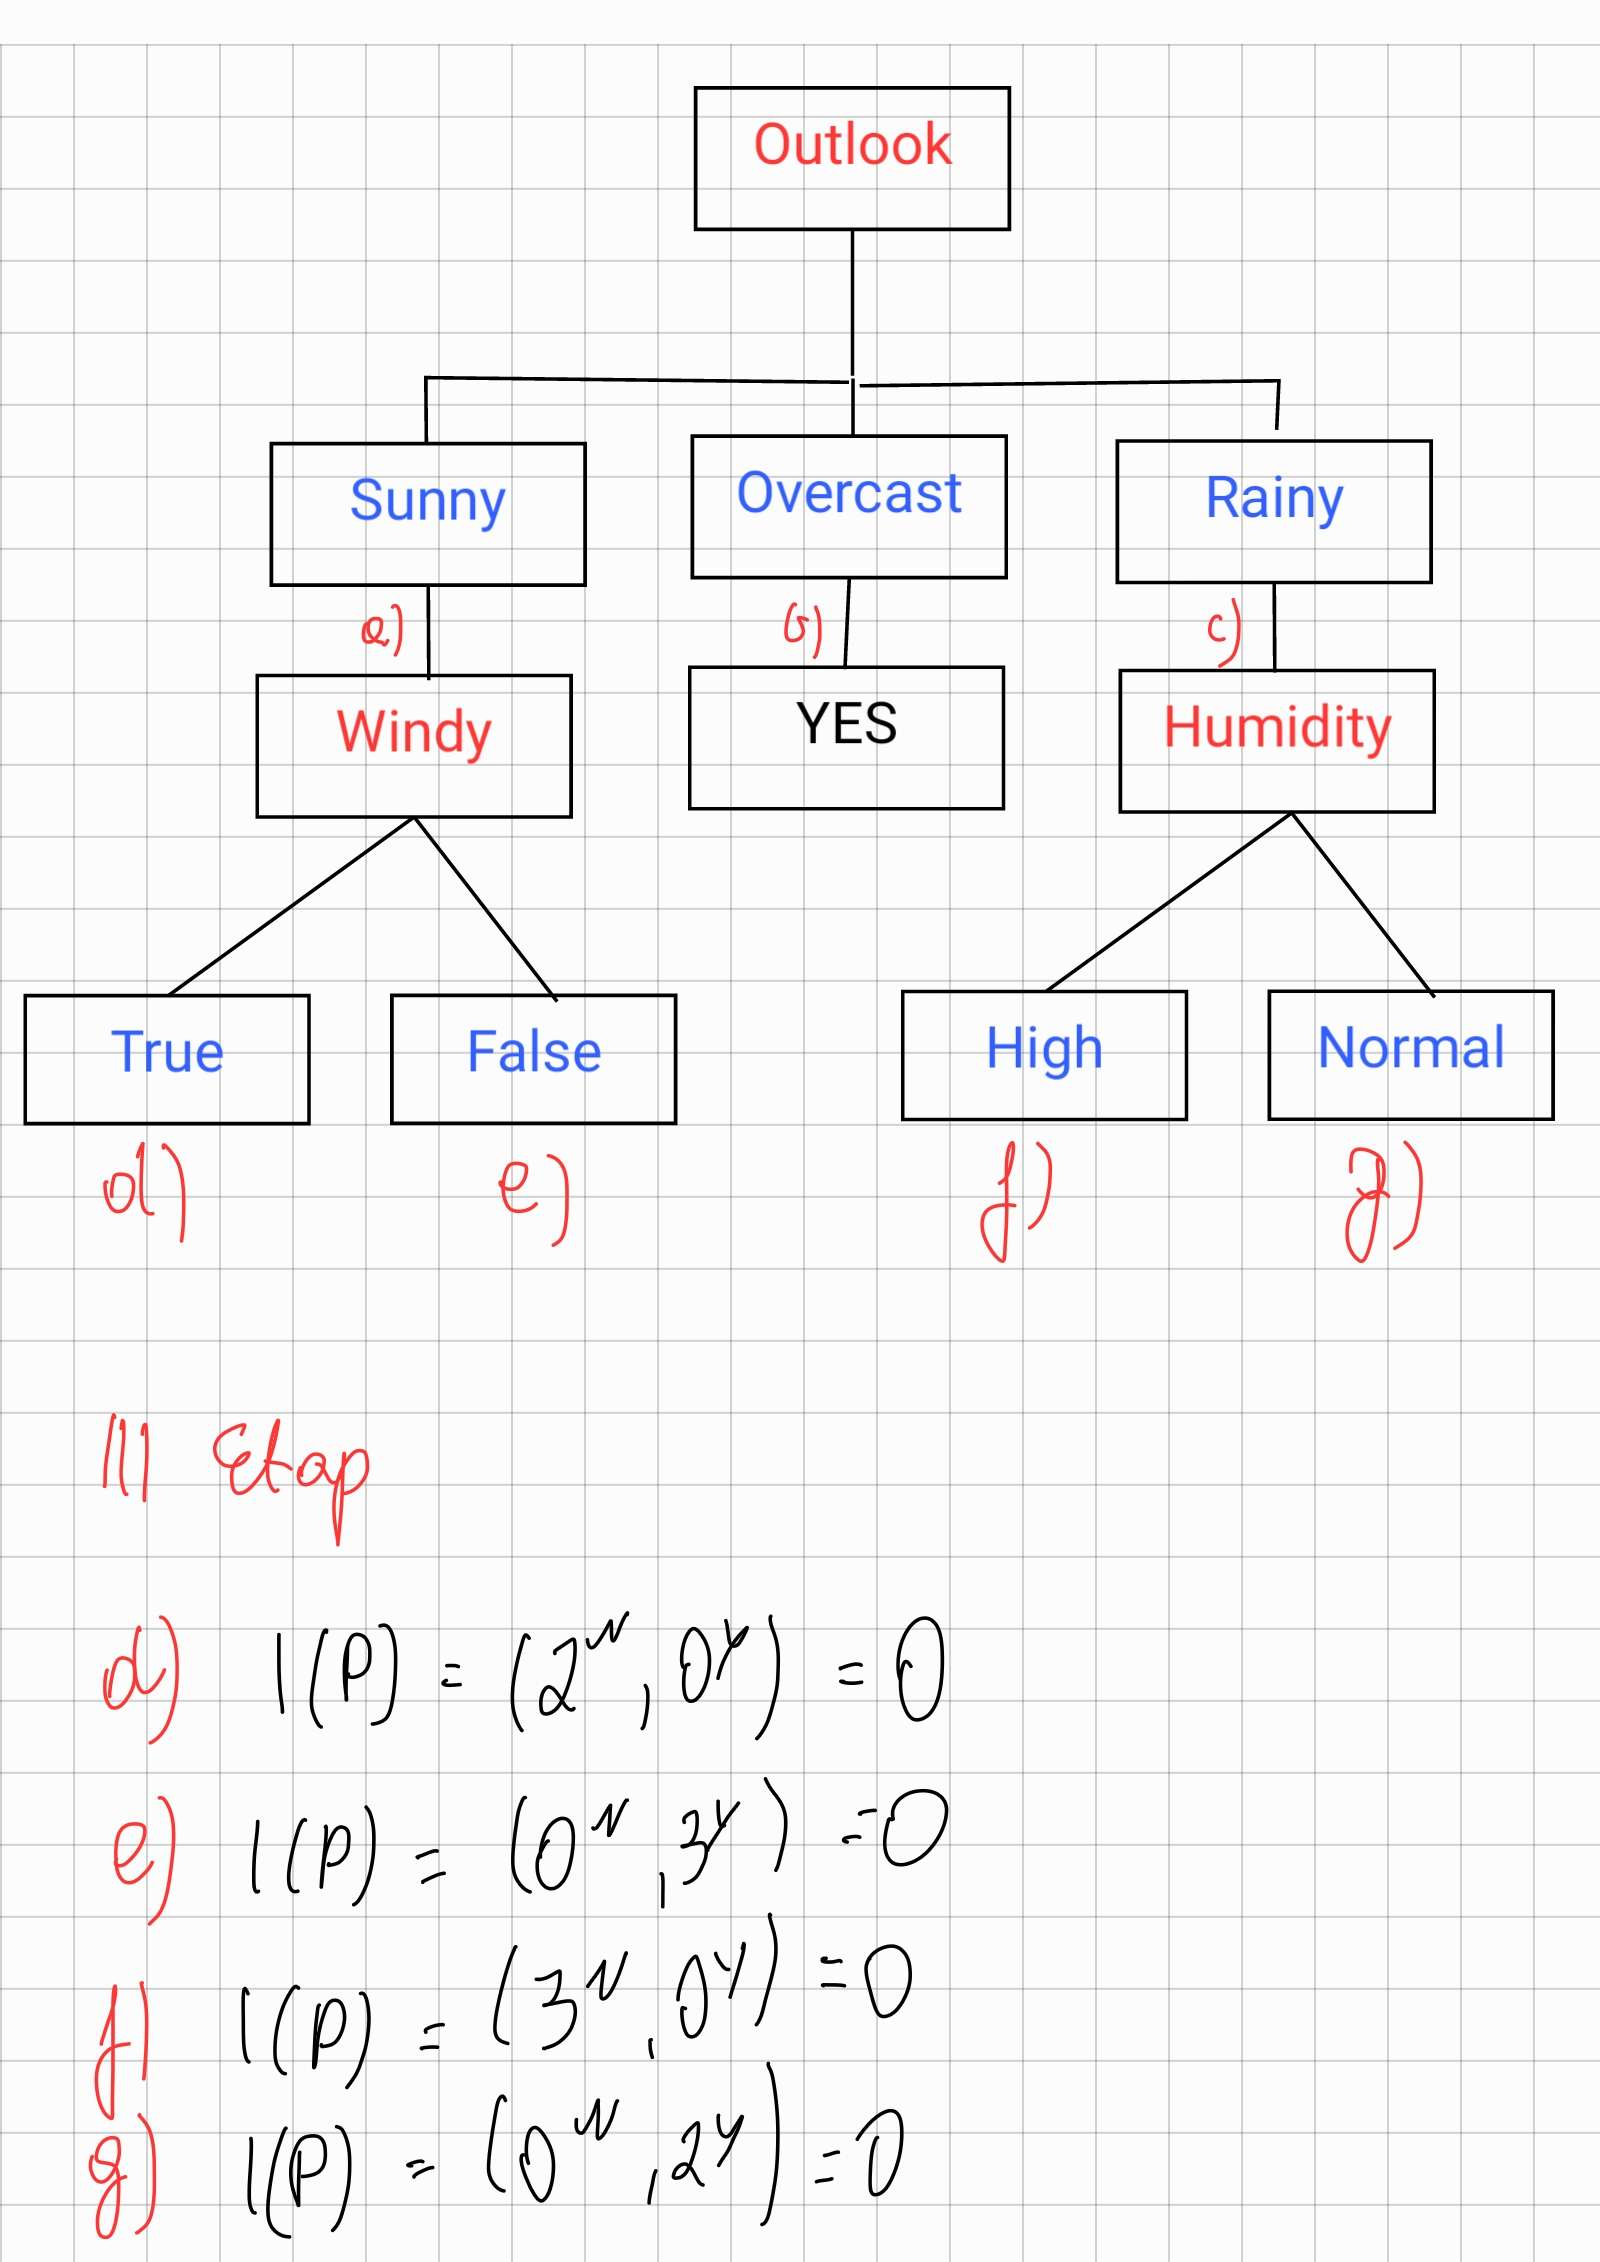
\includegraphics[width=\textwidth]{tree8.jpg}
\end{figure}

\begin{figure}[H]
    \centering
    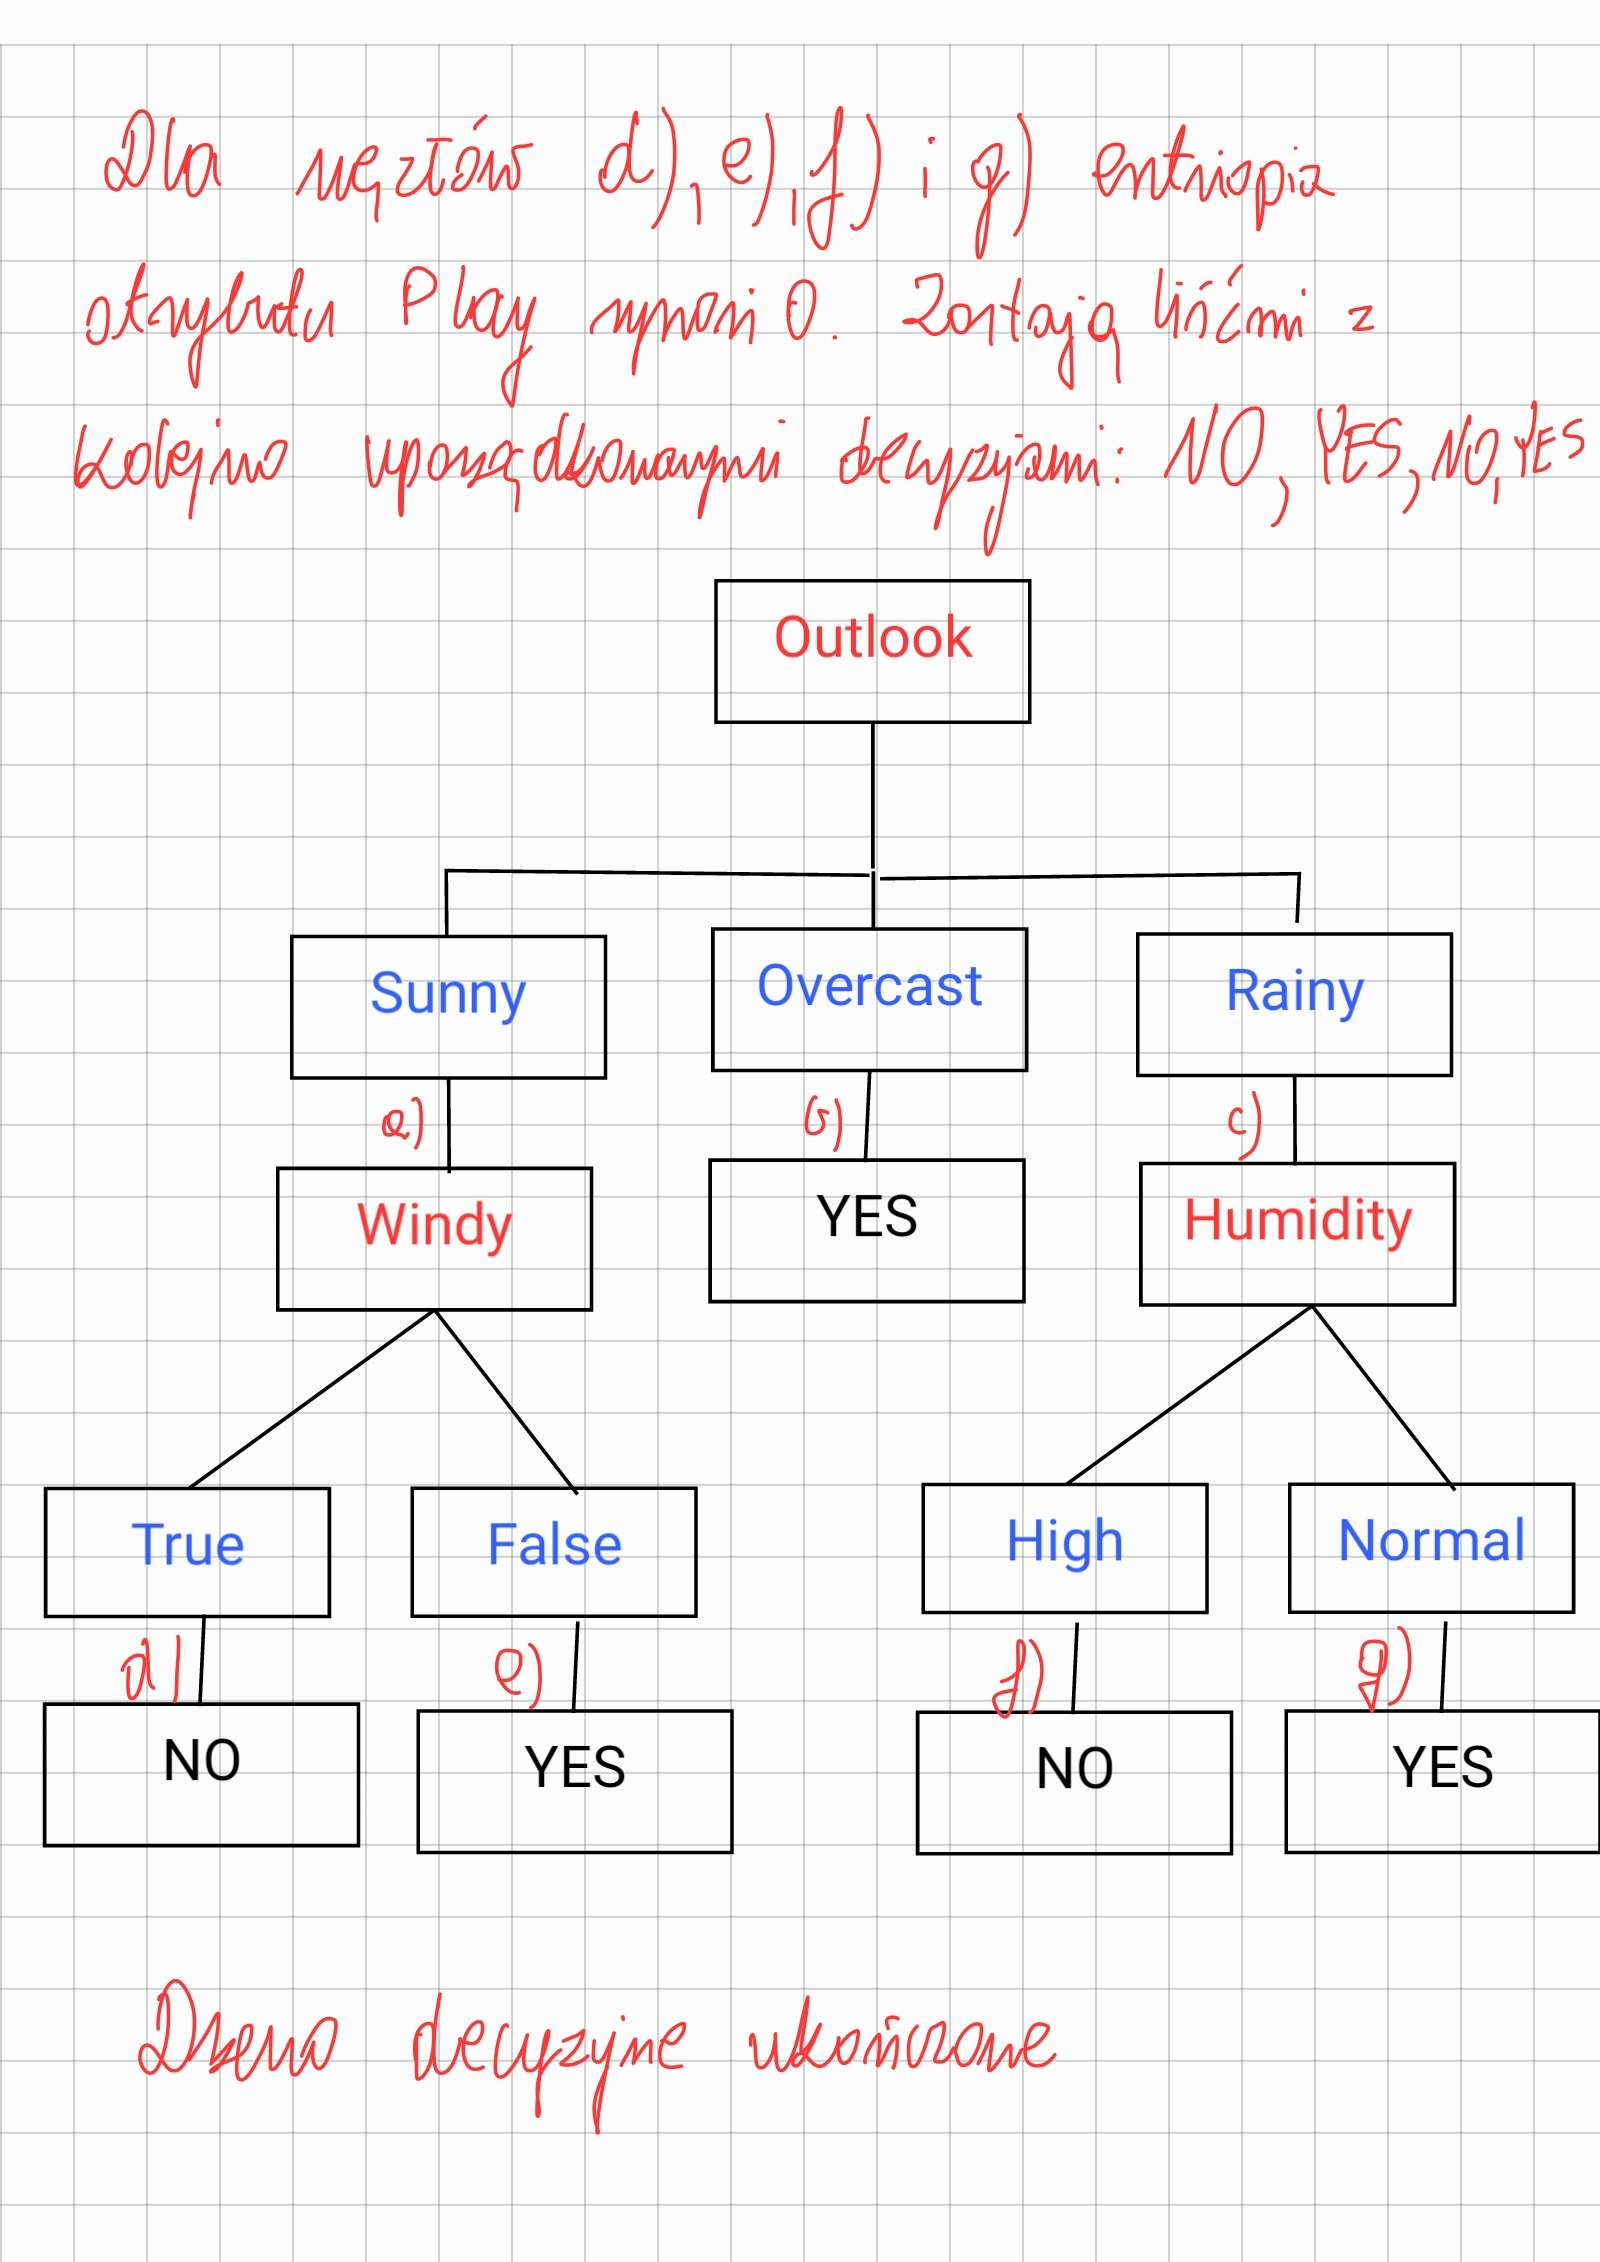
\includegraphics[width=\textwidth]{tree9.jpg}
\end{figure}


\end{document}